\hypertarget{app-lattice-generation}{%
\section{Lattice Generation}\label{app-lattice-generation}}

\hypertarget{graph-representation}{%
\subsection{Graph Representation}\label{graph-representation}}

Three key pieces of information allow us to represent amorphous lattices. The majority of the graph connectivity is encoded by an ordered list of edges \((i,j)\). These are ordered to represent both directed and undirected graphs. This is useful for defining the sign of bond operators \(u_{ij} = - u_{ji}\).

Information about the embedding of the lattice onto the torus is encoded into a point on the unit square associated with each vertex. The torus is unwrapped onto the square by defining an arbitrary pair of cuts along the major and minor axes. For simplicity, we take these axes to be the lines \(x = 0\) and \(y = 0\). We can wrap the unit square back up into a torus by identifying the lines \(x = 0\) with \(x = 1\) and \(y = 0\) with \(y = 1\).

Finally, we need to encode the topology of the graph. This is necessary because, if we are simply given an edge \((i, j)\) we do not know how the edge gets from vertex i to vertex j. One method would be taking the shortest path, but it could also `go the long way around' by crossing one of the cuts. To encode this information, we store an additional vector \(\vec{r}\) associated with each edge. \(r_i^x = 0\) means that edge i does not cross the x. \(r_i^x = +1\) (\(-1\)) means it crossed the cut in a positive (negative) sense.

This description of the lattice has a very nice relationship to Bloch's theorem. Applying Bloch's theorem to a periodic lattice essentially means wrapping the unit cell onto a torus. Variations that happen at longer length scales than the size of the unit cell are captured by the crystal momentum. The crystal momentum inserts a phase factor \(e^{i \vec{q}\cdot\vec{r}}\) onto bonds that cross to adjacent unit cells. The vector \(\vec{r}\) is exactly what we use to encode the topology of our lattices.

\hypertarget{fig:bloch}{%
\begin{figure}
\centering
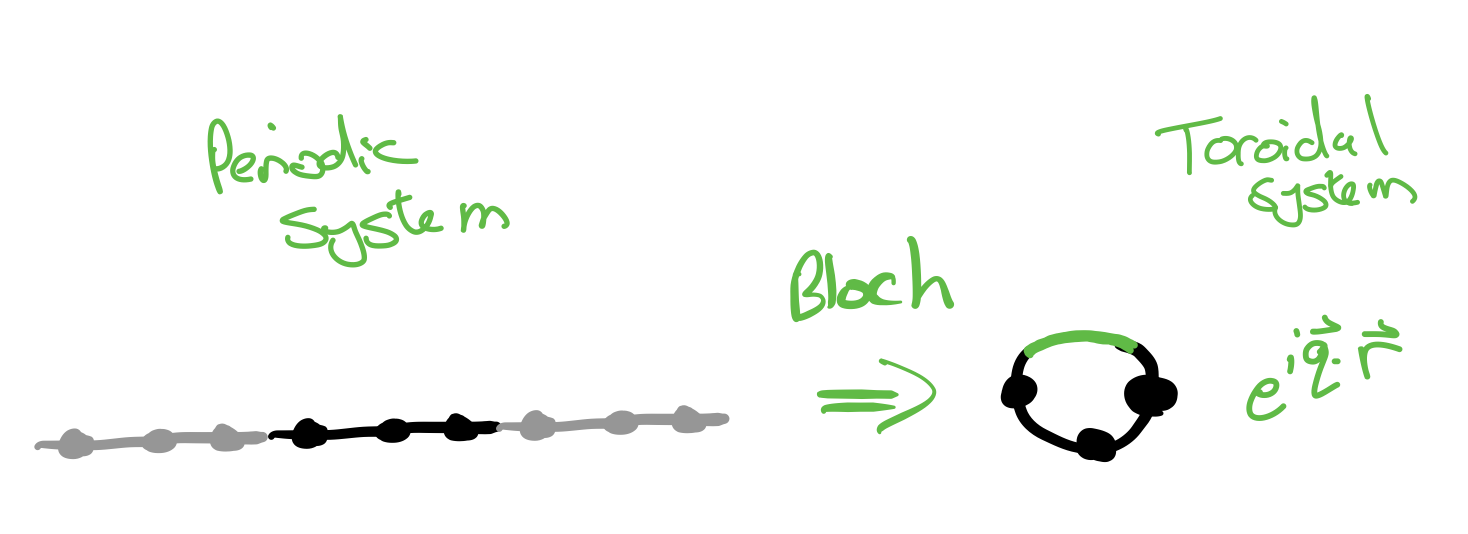
\includegraphics[width=1\textwidth,height=\textheight]{figure_code/amk_chapter/methods/bloch.png}
\caption[{Bloch's Theorem and the Torus}]{Bloch's theorem can be thought of as transforming from a periodic Hamiltonian on the plane to the unit cell defined on a torus. In addition we get some phase factors \(e^{i\vec{k}\cdot\vec{r}}\) associated with bonds that cross unit cells that depend on the sense in which they do so \(\vec{r} = (\pm1, \pm1)\). Representing graphs on the torus turns out to require a similar idea, we unwrap the torus to one unit cell and keep track of which bonds cross the cell boundaries.}
\label{fig:bloch}
\end{figure}
}

\hypertarget{encoding-edge-colouring-problems-as-sat-instances}{%
\subsection{Encoding edge-colouring problems as SAT instances}\label{encoding-edge-colouring-problems-as-sat-instances}}

\hypertarget{fig:times}{%
\begin{figure}
\centering
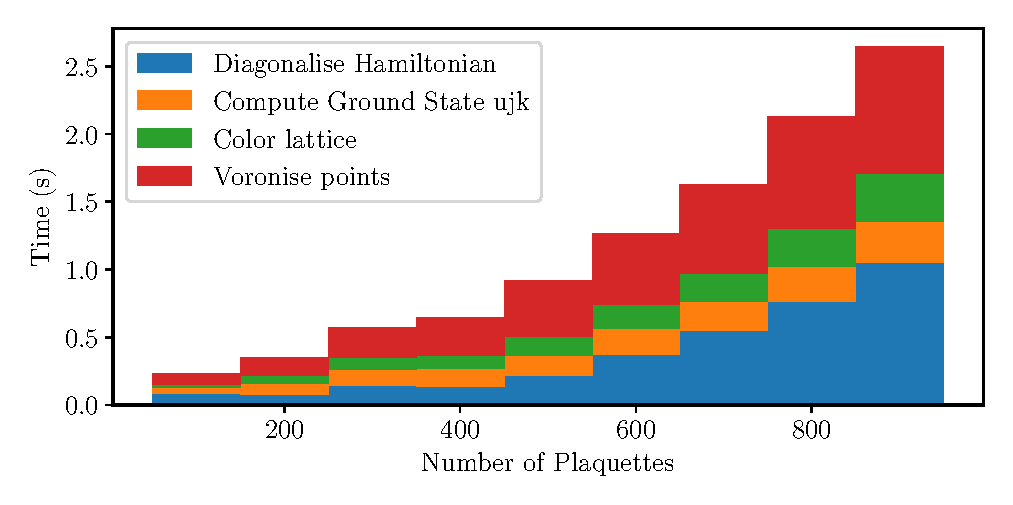
\includegraphics[width=1\textwidth,height=\textheight]{figure_code/amk_chapter/methods/times/times}
\caption[{Computation Time Spent on Different Procedures.}]{The proportion of computation time taken up by the four longest running steps when generating a lattice. For larger systems, the time taken to perform the diagonalisation dominates.}
\label{fig:times}
\end{figure}
}

In the main text we discuss the problem of three-edge-colouring, assigning one of three labels to each edge of a graph such that no edges of the same label meet at a vertex. To solve this in practice I use a solver called \passthrough{\lstinline!MiniSAT!}~\autocite{imms-sat18}. Like most modern SAT solvers, \passthrough{\lstinline!MiniSAT!} requires the input problem to be specified in Conjunctive Normal Form (CNF). CNF requires that the constraints be encoded as a set of \emph{clauses} of the form

\[x_1 \;\textrm{or}\; -x_3 \;\textrm{or}\; x_5,\]

that contain logical ORs of some subset of the variables where any of the variables may also be logically NOT'd, which we represent by negation here. A solution of the problem is one that makes all the clauses simultaneously true.

I encode the edge colouring problem by assigning \(3B\) boolean variables to each of the \(B\) edges of the graph, \(x_{i\alpha}\) where \(x_{i\alpha} = 1\) indicates that edge \(i\) has colour \(\alpha\). For edge colouring graphs we need two types of constraints: 1. Each edge is exactly one colour. 2. No neighbouring edges are the same colour.

The first constraint is a product of doing this mapping to boolean variables. The solver does not know anything about the structure of the problem unless it is encoded into the variables. Let's say we have three variables that correspond to particular edge being red \(r\), green \(g\) or blue \(b\). To require that exactly one of the variables be true, we can enforce that no pair of variables be true: \passthrough{\lstinline!-(r and b) -(r and g) -(b and g)!}

However, these clauses are not in CNF form. Therefore, we also have to use the fact that \passthrough{\lstinline!-(a and b) = (-a OR -b)!}. To enforce that at least one of these is true we simply OR them all together \passthrough{\lstinline!(r or b or g)!}

To encode the fact that no adjacent edges can have the same colour, we emit a clause that, for each pair of adjacent edges, they cannot be both red, both green or both blue.

We get a solution or set of solutions from the solver, which we can map back to a labelling of the edges.

The solution presented here works well enough for our purposes. It does not take up a substantial fraction of the overall computation time, see +fig:times but other approaches could likely work.

When translating problems to CNF form, there is often some flexibility. For instance, we used three boolean variables to encode the colour of each edge and then additional constraints to require that only one of these variables be true. An alternative method which we did not try would be to encode the label of each edge using two variables, yielding four states per edge, and then add a constraint that one of the states, say (true, true) is disallowed. This would, however, have added some complexity to the encoding of the constraint that no adjacent edges can have the same colour.

The popular \emph{Networkx} Python library uses a greedy graph colouring algorithm. It simply iterates over the vertices/edges/faces of a graph and assigns them a colour that is not already disallowed. This does not work for our purposes because it is not designed to look for a particular n-colouring. However, it does include the option of using a heuristic function that determine the order in which vertices will be coloured~\autocite{kosowski2004classical,matulaSmallestlastOrderingClustering1983}. Perhaps
